\section{Probabilistic Trace Alignment}
\texttt{\color{red}[TODO: introduction, motivation, and why it is useful to run it as a $k$-best search]}
\resizeableyellownote{3}{3}{
	Assuming that Rafael writes the definition of his ranking function, that can be expressed as $r(\tau^*,\tau)=d(\tau^*,\tau)w_\tau$ for a query trace $\tau^*$ and a trace $\tau\in\mathcal{W}_p^n(P)$
}

\subsection{Exact $k$-probabilistic Traces Alignment Problem}\label{subsec:exbkptap}
\texttt{\color{red}[TODO: the introduction of this section depends on how we want to formulate the problem. I suddenly start with the definition of the k-Nearest Neighbour, but I am aware that we need to provide first a bit of context]}

\begin{definition}[$k$-Nearest Neighbour]
Given a set of vectors\yellownote{Is this definition required, or an informal definition will do?}  $\mathcal{X}\subseteq \mathbb{R}^d$ within a $d$-dimensional Euclidean space and a query vector $q\in\mathbb{R}^d$, the $k$-nearest neighbour algorithm returns a subset $K\subseteq\mathcal{X}$ of $k$ elements minimizing the distance from $v$:
$$knn(k,q,\mathcal{X})=\begin{cases}
	\emptyset& k \leq 0\\
	\{c\}\cup knn(k-1,q,\mathcal{X}\backslash\{c\}) & k> 0 \Rightarrow c:={\arg\min}_{x\in\mathcal{X}}\|x-q\|_2\\
\end{cases}$$
\end{definition}

We can express our probabilistic trace match as finding the trace that maximizes both the trace's probability and its similarity with the query trace $\tau^*$. Still, the trace alignments problems are usually expressed via trace alignments cost functions, and not via trace similarities \cite{LeoniM17}. Given a generic trace cost function $d(\tau,\tau')$, it is always possible to convert it into a normalized similarity score $s_d(\tau,\tau'):=1/(d(\tau,\tau')/c+1)$ where $c\in\mathbb{N}_{\neq 0}$ is a constant, so that the maximum similarity of $1$ is reached when the distance is $0$ and the similarity decreases while the distance increases \cite{BergamiBM20}.

At this point, we can map each weighted trace  $\braket{\tau,w_\tau}\in\mathcal{W}_p^n(P)$ that we need to align with $\tau^*$ as a point $\tau\overset{\mu_{\tau^*}}{\mapsto}(w_\tau,\; s_d(\tau,\tau^*))$ in the 2-dimensional similarity/probability space, so that the trace finding problem reduces to find a data point maximising the product $ps$ (Figure \ref{fig:spp}).

\begin{table}[!t]
\centering
\caption{Expected ranking of the paths from Example \ref{ex:withpaths} with the trace $\tau^*=\textup{caba}$. The cost function is the one from \cite{LeoniM17} and its normalized similarity score has $c=5$.}\label{tab:expected}
\begin{tabular}{lc|ll|cl}
	\toprule
	
	\multirow{2}{*}{$\tau$} & 
	\multirow{2}{*}{$d(\tau,\tau^*)$} & 
	\multicolumn{2}{c|}{$\mu_{\tau^*}$} &
	 \multirow{2}{*}{$\approx s_d(\tau,\tau^*)\cdot w_\tau$} & \multirow{2}{*}{\textit{expected ranking}}\\
	 
	\cline{3-4} &&  $\langle w_\tau$ &  $,\,s_d(\tau,\tau^*)\rangle $ &&\\
	 
	\midrule
	{a}  & $3$ & $0.4$ & $\;\; 0.6250$  & $0.2500$ & \textbf{1}\\
	{aa}  & $2$ & $0.2$ & $\;\; 0.7142$ & $0.1428$ & \textbf{2}\\
	{aaa}  & $2$ & $0.1$ & $\;\; 0.7142$ & $0.0714$ & \textbf{3}\\
	{ca}  & $2$ & $0.07$ & $\;\; 0.7142$ & $0.0500$ & \textbf{4}\\
	{cb}  & $2$ & $0.06$ & $\;\; 0.7142$ & $0.0428$ & \textbf{5}\\
	{aaaa}  & $3$ & $0.05$ & $\;\; 0.7142$ & $0.0357$ & \textbf{6}\\
	{caa}  & $1$ & $0.035$ & $\;\; 0.8333$ & $0.0292$ &  \textbf{7}\\
	{caaa}  & $1$  & $0.0175$ & $\;\; 0.8333$ & $0.0145$ & \textbf{8}\\
	\bottomrule
\end{tabular}
\end{table}
\begin{example}\label{ex:rankingTaus}
Table \ref{tab:expected} represents the expected exact alignment raking of all the weighted traces $\braket{\tau,w_\tau}\in\mathcal{W}_0^4(P)$ generated by the PPN $P$ in Figure \ref{3figs} with a trace $\tau^*=\textup{caba}$.  Albeit traces \textit{caa} and \textit{caaa} are the most similar with \textit{caba}, their associated trace probability is $w_\tau$ is rather low, so traces having higher probability but lower similarity score are preferred (e.g., \textit{a} and \textit{aa}). Given that users might still prefer the most similar ones to the ones maximising both probability and similarity, we prefer to offer the user the whole set of the best $k$ solutions rather than cherry picking the best solution maximising both probability and similarity.
\end{example}

 At this stage, we can reduce the problem into a $k$-Nearest Neighbour search by providing a transformation $t$ such that the distance of $t(p,s)$ towards an arbitrary query point, e.g. the origin of the axes $\vec{0}$, corresponds to $\sfrac{1}{ps}$, so the transformed data points maximising $ps=k$ are all at the same distance $\sfrac{1}{k}$ from $\vec{0}$ (Figure \ref{fig:knnspace}). A possible transformation is the following:
\[t(p,s):=\left(\frac{1}{s\sqrt{p^2+s^2}},\; \frac{1}{p\sqrt{p^2+s^2}}\right)\]

\begin{example}
Figure \ref{fig:spp} shows a family of hyperbolae $ps=k$ describing all the points $(p,s)$ having $k$ as a weighted similarity score. For example,  point $\color{red}(1,1)$ represents the best possible trace match, as it means that there exists a trace $\braket{\tau,p}\in\mathcal{W}_p^n(P)$ with probability $p=1$ and trace similarity $s_d(\tau,\tau^*)=1$.

Figure \ref{fig:knnspace} shows that the transformation $t$ moves the points of the hyperbola $ps=k$ over a circumference $\overline{p}^2+\overline{s}^2=\sfrac{1}{k^2}$ describing a locus of the points equidistant from the origin of the axes $(0,0)$ with distance $\sfrac{1}{k}$. %This implies that now all the points $(p,s)$ having the same product $ps=k$ are equidistant from the origin of the axes, thus implying that we might now rank the points using a $k$-Nearest Neighbour algorithm using $q=\vec{0}$ as a query vector. 
This consideration will be formally proved in the subsequent lemma.
\end{example}

\begin{figure}[!t]
	\centering
	\subfloat[The similarity/probability space.]{\label{fig:spp}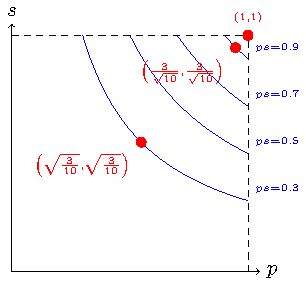
\includegraphics{images/original_space.pdf}}\qquad
	\subfloat[The transformed space for the $k$ nearest neighbours problem.]{\label{fig:knnspace}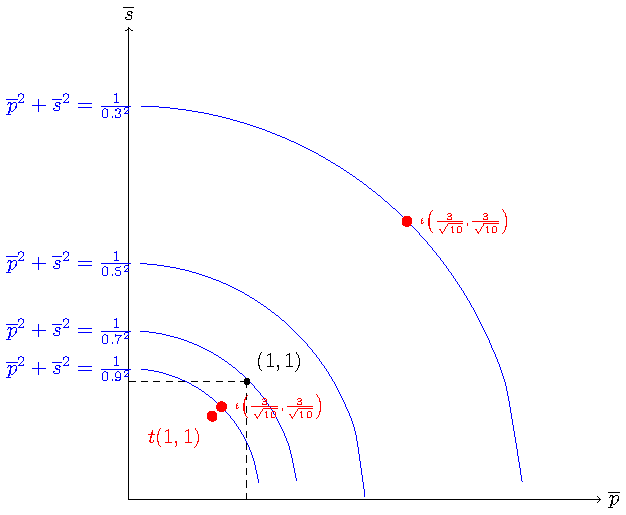
\includegraphics[scale=0.55]{images/transformed_space.pdf}}\\
	\caption{Two different characterizations of the probabilistic trace alignment problem. The best possible match is represented in red in both the similarity/probability space and in the transformed one.}
\end{figure}


 We can show with the next lemma that the following transformation is the one reducing the problem to the $k$-Nearest Neighbour problem:



\begin{lemma}
Given a value $k\in[0,1]\subseteq \mathbb{R}^+_0$, the set of points having the product $ps$ at least $k$ corresponts to the set of $t$-transformed points having a distance of at least $1/k$ from the origin of the axes.
\end{lemma}
\begin{proof}
\[\begin{aligned}
ps\geq k&\Leftrightarrow \frac{1}{ps}\leq\frac{1}{k} \\
	   &\Leftrightarrow \frac{\sqrt{p^2+s^2}}{ps\sqrt{p^2+s^2}}\leq\frac{1}{k} \\
	   &\Leftrightarrow \sqrt{\frac{p^2+s^2}{p^2s^2(p^2+s^2)}}\leq\frac{1}{k} \\
	   &\Leftrightarrow \sqrt{\frac{p^2}{p^2s^2(p^2+s^2)}+\frac{s^2}{p^2s^2(p^2+s^2)}}\leq\frac{1}{k} \\
	   &\Leftrightarrow \sqrt{\frac{1}{s^2(p^2+s^2)}+\frac{1}{p^2(p^2+s^2)}}\leq\frac{1}{k} \\
	   &\Leftrightarrow \left\|{\biggr({\frac{1}{s\sqrt{p^2+s^2}},\frac{1}{p\sqrt{p^2+s^2}}\biggr)}-\vec{0}}\right\|_2\leq\frac{1}{k} \\
	   &\Leftrightarrow \left\|t(p,s)-\vec{0}\right\|_2\leq\frac{1}{k} \\
\end{aligned}\]
\end{proof}
\begin{lemma}
Given a Petri Net $P$ and a trace $t^*$, the probabilistic trace alignment problem of the best $k$ traces reduces to the $k$-Nearest Neighbour problem $\mu_{\tau^*}^{-1}(knn(k,\vec{0},\mu_{\tau^*}(\mathcal{W}_0^{\aleph_0}(P))))$.
\end{lemma}
\begin{proof}
Trivial by definition of $\mu_{\tau^*}$ and for the previous lemma.
\end{proof}

\begin{table}[!t]
\centering
\caption{Representing the point from Table \ref{tab:expected} in the transformed space.}\label{tab:transf}
\begin{tabular}{ll|lll}
	\toprule
	
	$\tau$ & $t(\mu_{\tau^*}(\tau))$ & $\norm{t(\mu_{\tau^*}(\tau))-\vec{0}}{2}$ & $\frac{1}{\norm{t(\mu_{\tau^*}(\tau))-\vec{0}}{2}}$ & \textit{distance ranking}\\
	
	\midrule	
	a   & $\braket{2.16, \;\,3.37}$ & $4.00$ & $0.2500$ & \textbf{1}\\
	{aa}  & $\braket{1.89, \;\,6.74}$ & $7.00$ & $0.1428$ & \textbf{2}\\
	aaa   & $\braket{1.94, 13.87}$ & $14.00$ & $0.0714$ & \textbf{3}\\
	ca   & $\braket{1.95, 19.91}$ & $20$ & $0.0500$ & \textbf{4}\\
	{cb}  & $\braket{1.95, 23.25}$ & $23.33$ & $0.0428$ & \textbf{5}\\
aaaa   & $\braket{1.95, 27.93}$ & $28.00$ & $0.0357$ & \textbf{6}\\
caa   & $\braket{1.44, 34.26}$ & $34.29$ & $0.0292$ & \textbf{7}\\
caaa   & $\braket{1.44, 68.56}$ & $68.57$ & $0.0145$ & \textbf{8}\\
	\bottomrule
\end{tabular}
\end{table}
\begin{example}
We now want to show the correctness of the former lemmas with some examples. 
Table \ref{tab:transf} represents the transformed points $t(\mu_{\tau^*}(\tau))$ from the data points $\mu_{\tau^*}(\tau)$  calculated  Example \ref{ex:rankingTaus}. The third column shows the distance of the transformed point from the origin: the following column shows that the inverse of such distance exactly represents the previously calculated $s_d(\tau,\tau^*)\cdot w_\tau$, thus empirically implying that the $k$-nearest neighbours problem corresponts to the best $k$ traces maximising the product $s_d(\tau,\tau^*)\cdot w_\tau$.
\end{example}





At this stage, we can possibly solve the $k$-probabilistic trace alignment problem by generating a new instance of the $k$-Nearest Neighbour problem for each possible trace $\tau^*$ that we want to align towards the traces coming from a PPN. On the other hand, this solution might result quite costly, as solving the problem would require either to use a brute force search algorithm or to load and index our set of points each time.\yellownote{TODO: add references and explaination to the problem (we need a Related Work section\dots? I am accustumed to write such sections.)} In the next section we will discuss an approximated version of the problem providing a trade off between accuracy and efficiency.


\subsection{Approximate $k$-probabilistic Traces Alignment Problem}\label{subsec:akptap}
\texttt{\color{red}[TODO: provide some context and introduction. I'm facing the same problem as in the previous subsection, as the content in here depends on some content that I do not know if I have to write or not\dots]}

Given the characterization of a PPN as in \S\ref{subsec:ppn} and the embedding strategy proposed in Definition \ref{def:ppne}, we can generate an embedding for each possible weighted trace $\braket{\tau,w_\tau}\in\mathcal{W}_p^n(P)$ for a given PPN $P$ as described in the following definition:
\begin{definition}[Trace Embedding for PPNs]
Given a minimum probability threshold $p$, a maximum path length $n$, and a PPN $P=(s,t,L,R,w)$, we generate the set of the trace embeddings for $P$ as follows:
\begin{enumerate}
	\item for each weighted trace $\braket{\tau,w_\tau}\in\mathcal{W}_p^n(P)$ generated from a path $\pi_\tau=s\to n_2\rightsquigarrow n_m\to t$ over $R$, we generate a PPN $P_\tau=(s',t',L_\tau,R_\tau,w_\tau)$, where \begin{alphalist}
		\item $s'=s$ if $\textit{label}(s)\neq \varepsilon$ and $t'=n_2$ otherwise,
		\item $t'=t$ if $\textit{label}(t)\neq \varepsilon$ and $t'=n_m$ otherwise,
		\item $L_\tau$ (and $R_\tau$) is the submatrix of $L$ (and $R$) over the non-$\varepsilon$ labelled notes in $\pi_\tau$ and the labels from $\tau$,
		\item $w'$ is initialised by $w$ and then multiplied by $[R]_{s,n_2}$ (and also $[R]_{n_m,t}$) if $\textit{label}(s)=\varepsilon$ (and  $\textit{label}(t)=\varepsilon$);
	\end{alphalist}
	\item each $P_\tau$ is then represented as $\phi_{\mathcal{P}}(P_\tau)$ and added to the set $\mathbf{T}_p^n(P)$.
\end{enumerate}
\end{definition}

\begin{table}[!t]
	\caption{Generating the sub-PPNs $P_\tau\in \mathbf{T}_0^4(P)$ from the PPN $P$ via the set of weighted traces $\mathcal{W}_0^4(P)$. $l$ and $w$ respectively represent the desired parameter for $\phi_{\mathcal{P}}(P_\tau)$ and the weight associated to $P_\tau$.}\label{tab:proj}
	\centering
	\begin{tabular}{>{\centering\arraybackslash} m{1cm}| >{\centering\arraybackslash} m{4cm} >{\centering\arraybackslash} m{1cm} >{\centering\arraybackslash} m{1cm} }
		\toprule
		$\tau$&$P_\tau$&$l$&$w$\\
		\midrule
		a & 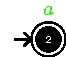
\includegraphics{images/trace_a} & $1$ & $\color{red}p_1p_6$\\   
		cb & 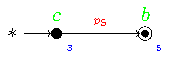
\includegraphics{images/trace_cb} & $2$ & $\color{red}p_2$\\
		aa & 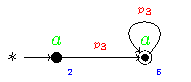
\includegraphics{images/trace_a_loop} & $2$ & $\color{red}p_1p_6$\\ 
		ca & 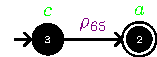
\includegraphics{images/trace_ca} & $2$ & $\color{red}p_2p_6$\\ 
		aaa & 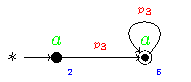
\includegraphics{images/trace_a_loop} & $3$ & $\color{red}p_1p_6$\\ 
		caa & 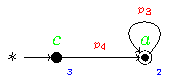
\includegraphics{images/trace_ca_loop} & $3$ & $\color{red}p_2p_6$\\  
		\begin{tabular}{l}aaaa\end{tabular} & 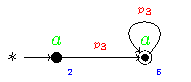
\includegraphics{images/trace_a_loop} & $4$ & $\color{red}p_1p_6$\\ 
		caaa & 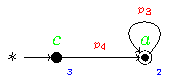
\includegraphics{images/trace_ca_loop} & $4$ & $\color{red}p_2p_6$\\  
		\bottomrule
	\end{tabular}
\end{table} \begin{table}[!t]
	\centering
	\caption{Embedding for all the traces of maximum length $4$ generated from $P$.}\label{tab:emb2}
	\begin{tabular}{l|l|l|l|l|l|l|}
		\toprule
		& a    & b                                                   & c    & aa   & ca   & cb   \\
		\midrule
		
		
		$\phi_{\mathcal{P}}(P_\textup{aaaa})$ & $1.00\cdot 10^{-24}$ & $0.00\cdot 10^{0}$ & $0.00\cdot 10^{0}$& $6.44\cdot 10^{-26}$& $0.00\cdot 10^{0}$& $0.00\cdot 10^{0}$\\
		$\phi_{\mathcal{P}}(P_\textup{aaa})$ & $1.00\cdot 10^{-24}$ & $0.00\cdot 10^{0}$ & $0.00\cdot 10^{0}$& $1.29\cdot 10^{-25}$& $0.00\cdot 10^{0}$& $0.00\cdot 10^{0}$\\
		$\phi_{\mathcal{P}}(P_\textup{aa})$ & $1.00\cdot 10^{-24}$ & $0.00\cdot 10^{0}$ & $0.00\cdot 10^{0}$& $2.57\cdot 10^{-25}$& $0.00\cdot 10^{0}$& $0.00\cdot 10^{0}$\\
		$\phi_{\mathcal{P}}(P_\textup{a})$ & $1.00\cdot 10^{-4}$ & $0.00\cdot 10^{0}$ & $0.00\cdot 10^{0}$& $0.00\cdot 10^{0}$& $0.00\cdot 10^{0}$& $0.00\cdot 10^{0}$\\
		$\phi_{\mathcal{P}}(P_\textup{caa})$ & $7.07\cdot 10^{-25}$ & $0.00\cdot 10^{0}$ & $7.07\cdot 10^{-25}$& $1.46\cdot 10^{-25}$& $2.05\cdot 10^{-25}$& $0.00\cdot 10^{0}$\\
		$\phi_{\mathcal{P}}(P_\textup{ca})$ & $7.07\cdot 10^{-25}$ & $0.00\cdot 10^{0}$ & $7.07\cdot 10^{-25}$& $0.00\cdot 10^{0}$& $1.00\cdot 10^{-8}$& $0.00\cdot 10^{0}$\\
		$\phi_{\mathcal{P}}(P_\textup{cb})$ &  $0.00\cdot 10^{0}$ & $7.07\cdot 10^{-25}$ & $7.07\cdot 10^{-25}$& $0.00\cdot 10^{0}$&  $0.00\cdot 10^{0}$ & $4.29\cdot 10^{-9}$\\
		$\phi_{\mathcal{P}}(P_\textup{caaa})$  & $7.07\cdot 10^{-25}$ &  $0.00\cdot 10^{0}$ & $7.07\cdot 10^{-25}$& $1.03\cdot 10^{-25}$&  $7.20\cdot 10^{-26}$ & $0.00\cdot 10^{0}$\\
		\bottomrule
	\end{tabular}
\end{table}
\begin{example}\label{ex:explainembed}
	Table \ref{tab:proj} represents the PPNs $P_\tau\in\mathbf{T}_p^n(P)$ with weight $w$ generated for each weighted path $\braket{\tau,w_\tau}\in \mathcal{W}_0^4(P)$ of length $l=|\tau|$ from the PPN $P$ in Figure \ref{fig:closed}. The associated weight $w$ derives from the source's outgoing edges (and target's ingoing edges) when such node is  labelled as $\varepsilon$: given that the selection of a trace $\tau$ implies performing a set of specific probabilistic choices, we can remove all the edges starting (and arriving) at nodes that are $\varepsilon$-labelled and move their score as the weight of the PPN. 
	
	Table \ref{tab:emb2} represents the embeddings $\phi_{\mathcal{P}}(P_\tau)$ generated from the sub-PPNs $P_\tau\in \mathbf{T}_0^4(P)$ of $P$, where the $l$ parameters required to compute $\epsilon$ via Equations \ref{eq:epsilon} and \ref{eq:nu} are the same as above. As we can see, this representation is completely independent from the representation associated to a trace to be aligned, and therefore it doesn't have to be recomputed at each alignment with a different $\tau^*$.
\end{example}



\begin{table}[!t]
	\caption{Comparison between the ranking induced by the kernel function and the expected ranking: the largest similar ranking subsequence is marked in blue.}\label{tab:rank3}
	\centering
	\begin{tabular}{l|c|ll}
		\toprule
		$\tau$ & $k_{\phi_{\mathcal{P}}}(\tau,\tau^*)$ & \textit{kernel ranking} & expected ranking\\
		\midrule
		a & $8.16\cdot 10^{-21}$ & \textbf{1} & \textbf{\color{blue}1}\\
		ca & $1.89\cdot 10^{-24}$ & \textbf{2} & \textbf{\color{blue}4}\\
		cb & $7.64\cdot 10^{-25}$ & \textbf{3} & \textbf{\color{blue}5}\\
		caa & $1.14\cdot 10^{-40}$ & \textbf{4} & \textbf{\color{blue}7}\\
		caaa & $9.84\cdot 10^{-41}$ & \textbf{5} & \textbf{\color{blue}8}\\
		aa & $9.28\cdot 10^{-41}$ & \textbf{6} & \textbf{\color{red}2}\\
		aaa & $8.72\cdot 10^{-41}$ & \textbf{7} & \textbf{\color{red}3}\\
		aaaa & $8.44\cdot 10^{-41}$ & \textbf{8} & \textbf{\color{red}6}\\
		
		\bottomrule
	\end{tabular}
\end{table}


At this stage, the computation of $\underset{\braket{\tau,w_\tau}\in \mathcal{W}_p^n(P), P_\tau\in\mathbf{P}_p^n(P)}{\max\arg} k_{\phi_\mathcal{P}}(P_\tau, T)$ returns the best approximated trace alignment $\tau$ for a query trace represented as $T$. Similarly, we can provide the PPN $P\in\mathbf{P}$ providing the best approximated alignment for $T$ as $\underset{P}{\max\arg}\underset{ P_\tau\in\mathbf{P}_p^n(P)}{\max} k_{\phi_\mathcal{P}}(P_\tau, T)$. 

\begin{example}
	Let us resume Example \ref{ex:explainembed}. 
	Given that $k_{\phi_{\mathcal{P}}}(\tau,\tau^*)=\braket{\phi_{\mathcal{P}}(P_\tau),\;\phi_{\mathcal{P}}(T)}$ for each weighted trace $\braket{\tau,w_\tau}\in\mathcal{W}_0^4(P)$, then the dot product between the resulting similarity ranking is represented in Table \ref{tab:rank3}. This similarity score approximates the expected ranking showed in Table \ref{tab:expected}, and tends to rank in similar ways the paths generated from the same subgraph of the PPN.
\end{example}


\begin{example}\label{ex:moreskew}
	Let us suppose to change the probability distribution associated to the $P$'s edges, so that it becomes more skewed and that some traces are relatively more probable than others. Let us set $p_1=p_2=0.5$, $p_3=0.9$, $p_6=0.1$, $p_4=0.3$, and $p_5=0.7$, so that the initial choice is equiprobable but performing a loop is more probable than terminating the path. The other tuning parameters are kept the same as in Example \ref{ex:withpaths}. In this case, we generate the following set of weighted traces:
$$\begin{aligned}
	\mathcal{W}_0^4(P)=\{&\braket{cb,0.25},\braket{aa,0.03214},\braket{a,0.03125},\braket{aaa,0.02893},\\
	&\braket{aaaa,0.02603},\braket{caa,0.01125},\braket{ca,0.01071},\braket{caaa,0.01012}\}\\
\end{aligned}$$
	Let us also assume that we want to align these traces in a probabilistic way with the query $\tau^*=\textup{caba}$: the distance ($d$) and similarity ($s_d$) scores will be still the same, while the associated probabilities will vary. The expected ranking by multiplying weight with similarity is represented in Table \ref{tab:witherror}. 
	
	As a consequence of the different probability distribution associated to the edges, a different set of embedding will be generated for each trace of interest while the PPN $T$ associated to $\tau^*$ will be kept the same. Table \ref{tab:witherror} represents the ranking induced by the kernel $k_{\phi_{\mathcal{P}}}$ over this different set of vectors by ranking the traces in descendant order of $k_{\phi_{\mathcal{P}}}$. As we might notice, the more skewed edge probability  distribution introduced more errors in the ranking result: while the largest ranking subsequence (marked in blue) always starts from the best expected trace \textit{cb}, this element now appears in third position, and the position of traces \textit{caa} and \textit{aaaa} is swapped.  
 
\end{example}
\begin{table}[!t]
	\centering
	\caption{Expected ranking of the paths from Example \ref{ex:moreskew} with the trace $\tau^*=\textup{caba}$. The cost function is the one from \cite{LeoniM17} and its normalized similarity score has $c=5$. Traces are ranked by decreasing kernel $k_{\phi_{\mathcal{P}}}$ value: slight changes in the expected expected order are circled, the others are marked in red.}\label{tab:witherror}
	\begin{tabular}{lc|ll|cc|l}
		\toprule
		
		\multirow{2}{*}{$\tau$} & 
		\multirow{2}{*}{$d(\tau,\tau^*)$} & 
		\multicolumn{2}{c|}{$\mu_{\tau^*}$} &
		\multirow{2}{*}{$\approx s_d(\tau,\tau^*)\cdot w_\tau$} &
		\multirow{2}{*}{$k_{\phi_{\mathcal{P}}}(\tau,\tau^*)$}&
		\multirow{2}{*}{\textit{expected ranking}}\\
		
		\cline{3-4} &&  $\langle w_\tau$ &  $,\,s_d(\tau,\tau^*)\rangle $ && as\\
		
		\midrule
		{a}  & $3$ & $0.05$ & $\;\; 0.6250$  & $0.03125$ & $8.16497\cdot 10^{-16}$ & \textbf{\color{red}3}\\
		{ca}  & $2$ & $0.015$ & $\;\; 0.7142$ & $0.01071$ & $1.30623\cdot 10^{-18}$ & \textbf{\color{red}7}\\
		{cb}  & $2$ & $0.35$ & $\;\; 0.7142$ & $0.25000$ & $1.01399\cdot10^{-18}$ & \textbf{\color{blue}1}\\
		{aa}  & $2$ & $0.045$ & $\;\; 0.7142$ & $0.03214$ & $1.01894\cdot10^{-30}$ & \textbf{\color{blue}2}\\
		{aaa}  & $2$ & $0.0405$ & $\;\; 0.7142$ & $0.02893$ & $9.98696\cdot10^{-31}$ & \textbf{\color{blue}4}\\
		{caa}  & $1$ & $0.0135$ & $\;\; 0.8333$ & $0.01125$ & $9.96052\cdot10^{-31}$ & \textbf{\color{blue}\ding{177}}\\
		{aaaa}  & $3$ & $0.03645$ & $\;\; 0.7142$ & $0.02603$ & $9.80476\cdot10^{-31}$ & \textbf{\color{blue}\ding{176}}\\
		{caaa}  & $1$  & $0.01215$ & $\;\; 0.8333$ & $0.01012$ & $9.52398\cdot 10^{-31}$ & \textbf{\color{blue}8}\\
		\bottomrule
	\end{tabular}
\end{table}

In the next section, we propose a novel scoring function providing a numerical characterization for objetively comparing the two traces, while comparing such function to the well-known Spearman Correlation Index.